\documentclass[usepdftitle=false,green]{beamer}
\beamertemplatenavigationsymbolsempty
\usepackage{beamerthemesplit}
\usepackage{graphics}
\usepackage{float}

%\usepackage[frenchb]{babel}
\usepackage[T1]{fontenc}
\usepackage[utf8]{inputenc}
\usepackage{lmodern}

\usepackage{amssymb,amsmath}

\usepackage{enumerate, graphicx}
\usepackage{eurosym}
\usepackage{comment}
\usetheme{Warsaw}
%\usefonttheme{serif} 
\usecolortheme{lily}
\usepackage{ gensymb }
\useinnertheme[shadow=true]{rounded}
\useoutertheme{infolines}

\usepackage{enumitem}
\usepackage{color}
\usepackage{multicol}
  
    
\title[Projet HPC]{\textbf{Décision de finales d'échecs}}

\author[M. Caristan \& A. Fernandez]{Mathis \textsc{Caristan} \& Alexandre \textsc{Fernandez}}

\institute[]{\textsc{UPMC}}
\date{28 Mars 2017}
%\begin{comment}
\newcommand{\nologo}{\setbeamertemplate{logo}{}} % command to set the logo to nothing
\logo{%
  \vspace*{-5ex}\makebox[0.98\paperwidth]{%
    %%\includegraphics[width=1cm,keepaspectratio]{pics/lpnhe.jpeg}%
    \hfill%
    %%\includegraphics[width=1cm,keepaspectratio]{pics/ATLAS.png}
  }%
}
%\end{comment}

%\usepackage[sorting=none, style=numeric, hyperref=auto]{biblatex}


%Centrer la table des matières
\usepackage{varwidth}    
\usepackage{etoolbox}
\makeatletter
\patchcmd{\beamer@sectionintoc}{%
  \hbox{\vbox{%
    \def\beamer@breakhere{\\}%
    \beamer@tocact{\ifnum\c@section=#1\beamer@toc@cs\else\beamer@toc@os\fi}{section in toc}}}%
}{%
  \hbox{%
    \def\beamer@breakhere{}%
    \beamer@tocact{\ifnum\c@section=#1\beamer@toc@cs\else\beamer@toc@os\fi}{section in toc}}%
}{}{}
\makeatother 

%Numerotation sans appendix
 \usepackage{etoolbox}
\makeatletter
\preto{\appendix}{%
  \patchcmd{\beamer@continueautobreak}{\refstepcounter{framenumber}}{}{}{}}
\makeatother


\begin{document}

{\nologo
\begin{frame}
\titlepage
\end{frame}
}

 \begin{frame}
 \frametitle{Table des matières}
\begin{center}
\begin{varwidth}{\textwidth}
\tableofcontents[sectionstyle=show,subsectionstyle=hide] 
\end{varwidth}
\end{center}
 \end{frame}
 
\section{Implémentation}
	\subsection{OpenMP}
\begin{frame}
    %\frametitle{Le LHC}
        \begin{center}
        \begin{itemize}
            \item[$\bullet$] \textbf{Idée : } Paralléliser la boucle \texttt{for} dans \texttt{evaluate}
            \item[$\bullet$] Profondeur max : 2 $\longrightarrow$ \textasciitilde 30 noeuds
            \item[$\bullet$] Deux choix d'implémentations possibles
                \begin{itemize}
                    \item[a$\degree$)] \texttt{parallel for} (plus simple)
                    \item[b$\degree$)] \texttt{task} (plus efficace)
            \end{itemize}
        \end{itemize}
            \begin{figure}
                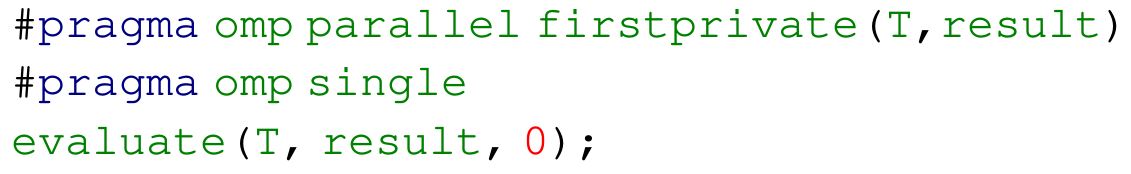
\includegraphics[scale=0.2]{pics/code1.png}
            \end{figure}
        \end{center}
\end{frame}

\begin{frame}
    \begin{center}
        \begin{figure}
            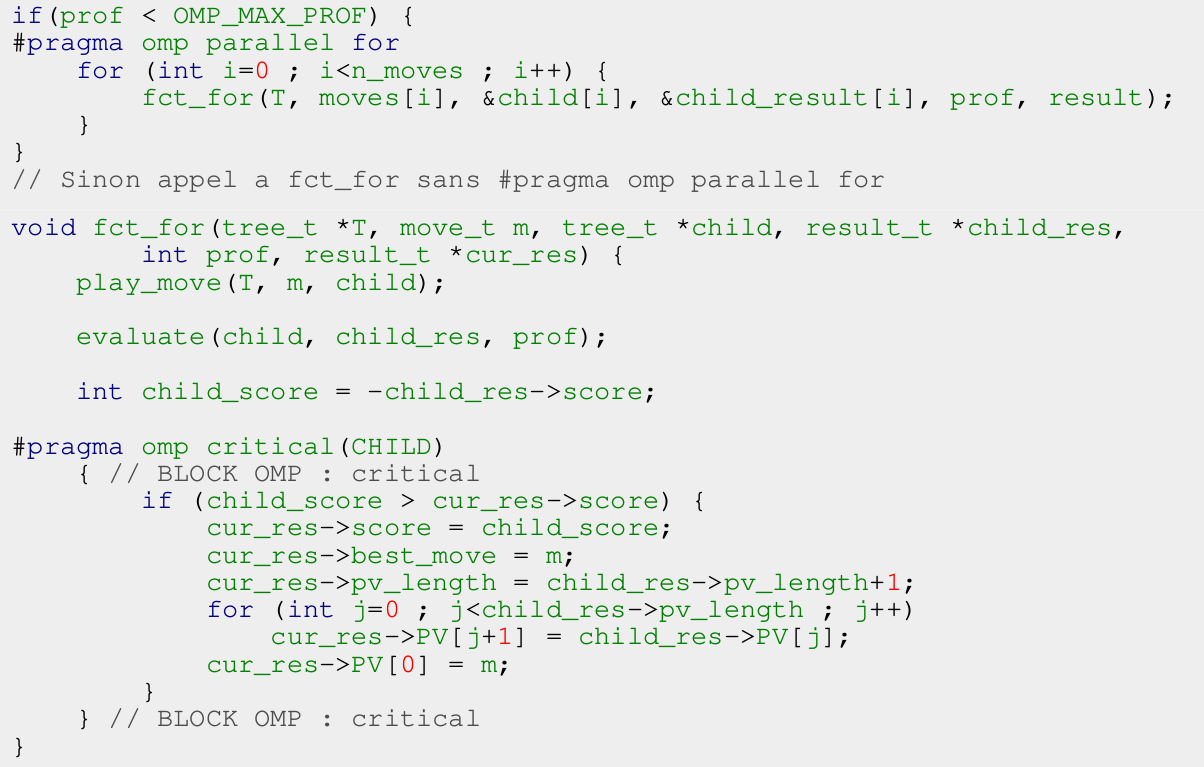
\includegraphics[scale=0.2]{pics/code2.png}
        \end{figure}
        \begin{itemize}
            \item[$\bullet$] Bloc \texttt{critical} pour protéger les accès concurents à cur\_res
            \item[$\bullet$] Factorisation du code dans la fonction \texttt{fct\_for}
        \end{itemize}
    \end{center}
\end{frame}


\begin{frame}
    \begin{itemize}
        \item[$\bullet$] \texttt{play\_move} et \texttt{evaluate} sont lancés dans des tâches
        \item[$\bullet$] Barrière de synchornisation à la fin du \texttt{for}
        \item[$\bullet$] La recherche du maximum est effectuée sur un tableau pour améliorer les performances
    \end{itemize}
    \begin{center}
        \begin{figure}
            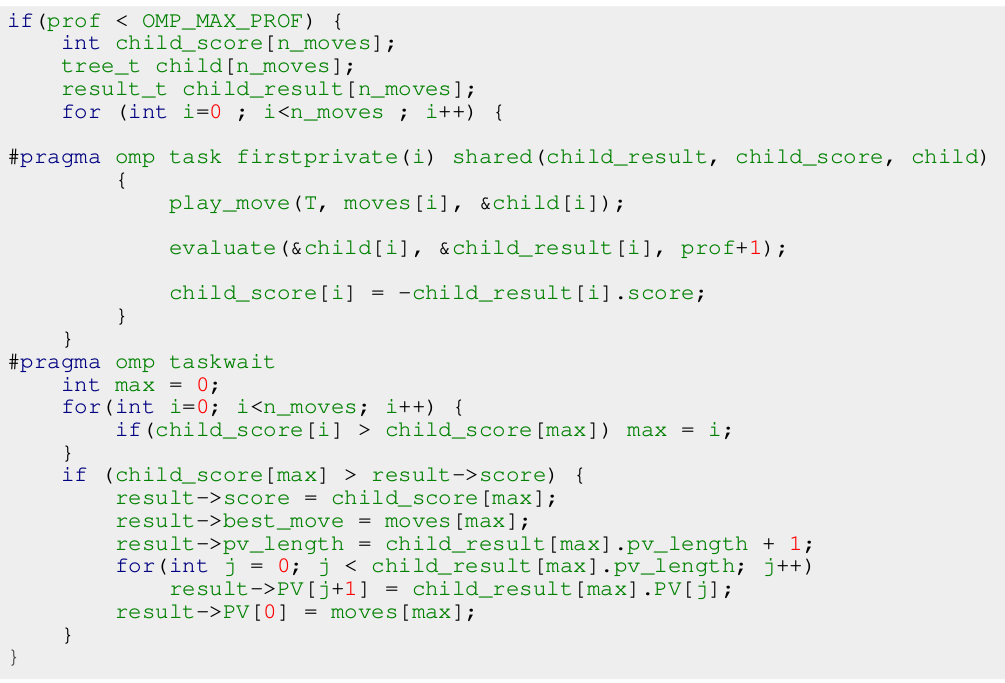
\includegraphics[scale=0.2]{pics/code3.png}
        \end{figure}
    \end{center}
\end{frame}

    \subsection{MPI}

\begin{frame}
    \begin{itemize}
        \item[$\bullet$] \textbf{Idée : } Atteindre une profondeur suffisante pour avoir une multiplicité de tâches intéressante.
        \item[$\bullet$] Pré-calcul (séquentiel) consistant à un parcours en largeur de l'arbre.
        \item[$\bullet$] \'Equilibrage de charge dynamique
        \item[$\bullet$] {\color{red} Réglages nécessaires selon les conditions d'utilisation}
    \end{itemize}
    \vspace{5ex}
    \begin{center}
        \begin{figure}
            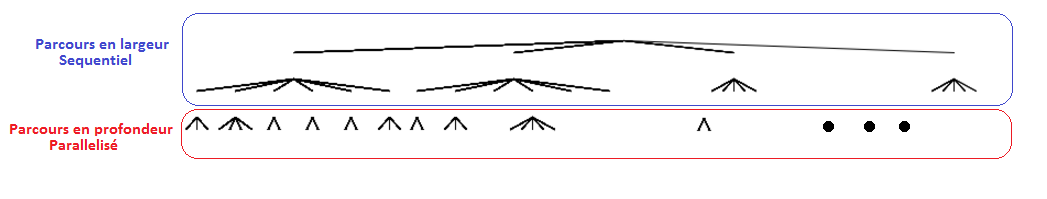
\includegraphics[scale=0.4]{pics/tree.png}
        \end{figure}
    \end{center}
\end{frame}

\begin{frame}
    \begin{center}
        \begin{figure}
            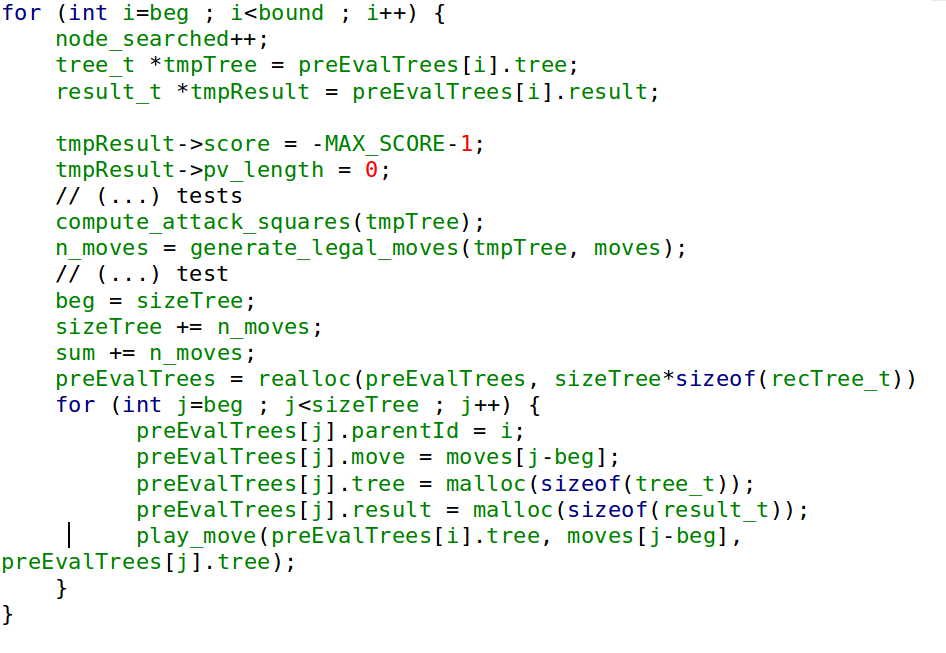
\includegraphics[scale=0.2]{pics/code4.png}
        \end{figure}
        \begin{itemize}
            \item[$\bullet$] La structure d'arbre des données est peu utilisée
            \item[$\bullet$] On remonte l'arbre au lieu de le descendre
            \item[$\bullet$] On ne garde une référence que vers le parent, pas les enfants
        \end{itemize}
    \end{center}
\end{frame}

\section{Perspectives et objectifs}

\begin{frame}
    \begin{center}
        \begin{itemize}
            \item[$\bullet$] \textbf{Idée : } Reprendre les principes de MPI et OpenMP en les combinant
            \item[$\bullet$] Utilisation d'OpenMP pour paralléliser le pré-calcul
            \item[$\bullet$] {\color{red} Pas encore implémenté}
        \end{itemize}
    \end{center}
\end{frame}



\begin{frame}
    \begin{center}
        \begin{figure}
            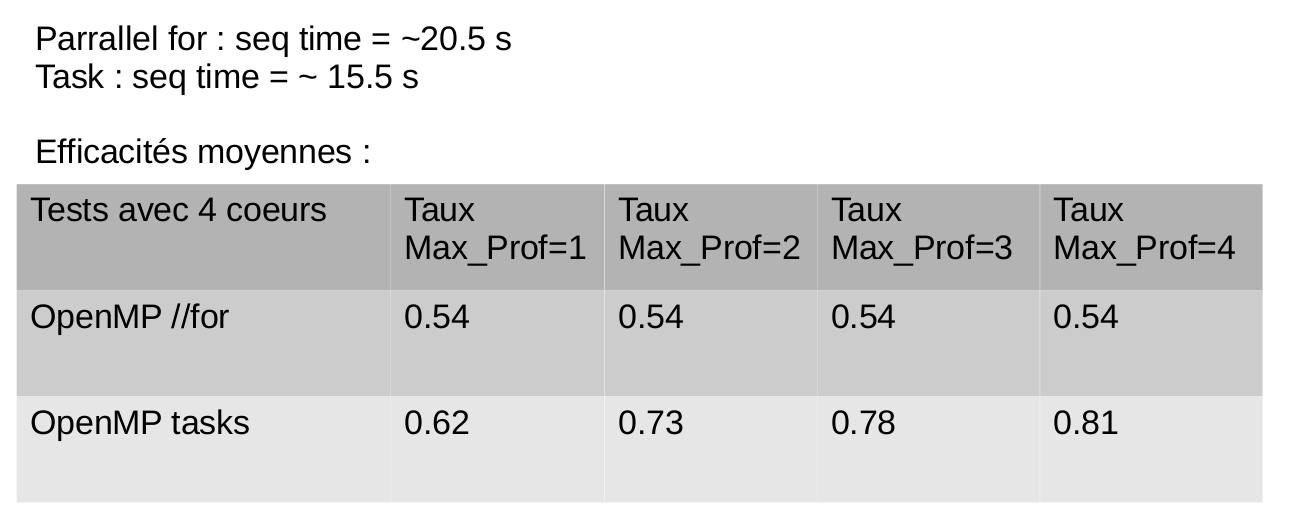
\includegraphics[scale=0.2]{pics/tab.png}
        \end{figure}
        \begin{itemize}
            \item[$\bullet$] On note une dépendance de plusieurs paramètres
            \item[$\bullet$] \textbf{Objectif : }Chercher à determiner la dépendance vis-à-vis des paramètres {\small (fit?)}
        \end{itemize}
    \end{center}
\end{frame}



\end{document}
